
\documentclass[a4paper,11pt]{article}
\usepackage{color}
\usepackage[T1]{fontenc}
\usepackage{fancyhdr}
\pagestyle{fancy}
\usepackage{ae}
% \usepackage[latin1]{inputenc}
\usepackage[brazil]{babel}
\usepackage[brazil]{hyperref}
\usepackage[alf]{abntex2cite}
\usepackage[utf8]{inputenc}
  
\usepackage{graphicx} 
\usepackage{url} 
\usepackage{lastpage}
\usepackage{multirow}
\usepackage{indentfirst}
\usepackage{amsmath}
\usepackage{siunitx}
\usepackage{booktabs}
\usepackage{pgfplots}
\usepackage{xifthen}
\usepackage{threeparttable}
\usepackage[version=3]{mhchem} % Formulas químicas automaticas, comando \ce{}
\usepackage{chemfig} % Formulas químicas automaticas, comando \ce{}
\usepackage{longtable}
\usepackage{pdflscape}
\usepackage{adjustbox}
\usepackage{multirow}
\usepackage{indentfirst}
\usepackage{lscape}
\usepackage{subfloat}
\usepackage{float}
\usepackage{subfig}
\usepackage{varwidth}
\newcommand{\subfigref}[1]{\hyperref[#1]{Figura~\ref*{#1}}}
\newcommand{\code}[1]{\texttt{#1}}

\sisetup{output-decimal-marker = {,}}
\newcommand{\theauthori}{}
\newcommand{\theauthorii}{}
\newcommand{\theauthoriii}{}
\renewcommand{\title}[1]{\newcommand{\thetitle}{#1}}
\renewcommand{\author}[1]{\newcommand{\theauthor}{#1}}
\newcommand{\authori}[1]{\renewcommand{\theauthori}{#1}}
\newcommand{\authorii}[1]{\renewcommand{\theauthorii}{#1}}
\newcommand{\authoriii}[1]{\renewcommand{\theauthoriii}{#1}}
\newcommand{\class}[1]{\newcommand{\theclass}{#1}}
\newcommand{\classProffessor}[1]{\newcommand{\theclassProffessor}{#1}}
\usepackage{palatino}
\renewcommand{\textsc}[1]{\fontshape{sc} \fontfamily{\sfdefault} \selectfont #1}

% o novo maketitlepage
\renewcommand{\maketitle}{
% Primeira página de título  
\pagestyle{empty}
\begin{center}
\textsc \large
Universidade Federal do Rio Grande do Sul \\
Escola de Engenharia \\
Departamento de Engenharia Química \\
Programa de Pós--Graduação em Engenharia Química
\vfill
\Large \textsc \theclass \\ Prof:~\theclassProffessor
\vfill \vfill
\huge \bfseries \textsc  
\thetitle
\vfill \vfill
%\begin{varwidth}[t]{\textwidth}
\Large \bfseries \textsc 
\theauthor\\
\ifthenelse{\equal{\theauthori}{}}{}{\theauthori\\}
\ifthenelse{\equal{\theauthorii}{}}{}{\theauthorii\\}
\ifthenelse{\equal{\theauthoriii}{}}{}{\theauthoriii}
%\end{varwidth}
\vfill \vfill 
\large \textsc Porto Alegre, RS \\ \today
\end{center}
\clearpage
\setcounter{page}{1}
\pagestyle{fancy} 
\lhead{}
} % end maketitle 

\begin{document}

\class{EQP 0015--Termodinâmica Aplicada a Processo de Separação}
\classProffessor{Paula Bettio Staudt}
\title{Trabalho 01}
\author{Eduaro Ribas}
% Para mais autores do trabalho, descomentar as linhas abaixo
\authori{Fabrício Ferrarini}
% \authorii{Aluno3}
% \authoriii{Aluno4}

% Capa
\maketitle  

% Incluir seções do trabalho
\section{Introdução Teórica}

\subsection{Modelo UNIFAC}

\citeonline{Fredenslund1975} explicam que a metodologia UNIFAC 
(“Universal Quasi-chemical Functional Activity Coefficient”)
é utilizável para uma vasta quantidade de misturas exibindo 
desvios positivos ou negativos da lei de Raoult. O método 
UNIFAC segue o modelo “Analytical-Solution-of-Groups”, ou ASOG,
de \citeonline{Derr1969}, onde os coeficientes de atividade
em misturas são relacionados ás interações entre os 
grupos estruturais. Além disso, o método UNIFAC pode 
ser usado para prever os coeficientes de atividade para 
os componentes em misturas binárias desconhecidas que
fazem parte de um determinado sistemas multicomponentes. 
Tais previsões podem ser utilizadas na geração de parâmetros
 binários em qualquer modelo de excesso de Gibbs.

%\apudonline{Fredenslund1975}{Fredenslund1975} 

\citeonline{Pollmann1996} citam que o logaritmo do coeficiente de
atividade em uma mistura é calculado (\autoref{eq:001}) via o somatório de duas
contribuições:
a combinatorial, devido aos diferentes tamanhos e formatos das moléculas, e a
residual representa a contribuição via interação energética entre as
moléculas. A relação que descreve tal somatório é:
\begin{equation}\label{eq:001}ln\gamma_i = ln\gamma_i^C +
ln\gamma_i^R\end{equation}
onde
$ln\gamma_i^C$ é o termo combinatório e $ln\gamma_i^R$ 
é o termo residual.


Todavia, \citeonline{Gmehling1996} cita que resultados não  
satisfatórios são obtidos para
sistemas cujos componentes detêm tamanhos bem diferentes, bem
como para coeficientes de atividade à diluição infinita. 
Assim, \citeonline{Muzenda2013} afirma que diferentes modificações 
foram propostas para os termos combinatorial e residual, 
bem como uma introdução da dependência da temperatura na 
interação dos parâmetros dos grupos funcionais.

\citeonline{Nagata1981} propuseram modificações apenas no termo residual
adicionando um termo tipo Flory-Huggins na relação de $ln\gamma_i^R$. 
Ademais, alterou a relação para com a fração de área 
superficial, utilizado originalmente, para dependência 
da fração molar do grupo funcional, além de relacionar o 
parâmetro de interação dos grupos funcionais com a 
temperatura. Entretanto, os resultados obtidos foram 
similares ao UNIFAC original, além de não haver grande 
evolução nos problemas encontrados no modelo original.

\citeonline{Larsen1987} propuseram modificações na expressão 
combinatorial do
UNIFAC original incorporando as modificações propostas por 
\citeonline{Kikic1980} e investigadas por \citeonline{Alessi1982}. 
O termo combinatorial tornou-se dependente do parâmetro de 
fração volumétrica do grupo funcional. O termo residual teve 
apenas modificação na interação com a temperatura. Como 
resultado, o modelo proposto obteve melhorias nas predições 
de equilíbrios líquido-vapor (VLE).

\citeonline{Weidlich1987} publicaram outro modelo modificado do
UNIFAC original, denominando-o de UNIFAC (Dortmund). Dentre as 
incorporações, destacam-se: a utilização dos parâmetros de 
volume e área superficial de van der Waals para alcanos 
cíclicos e reclassificação dos álcoois em primário, 
secundário e terciário com seus próprios parâmetros de 
volume e área superficial de van der Waals; e a extensão 
do ajuste dos parâmetros de interação dos grupos funcionais 
para inclusão dos coeficientes de atividade à diluição 
infinita, equilíbrios líquido-vapor e entalpia em excesso, 
buscando aprimorar a precisão de tais parâmetros.

Mais modelos baseados originalmente no UNIFAC de \citeonline{Fredenslund1975} são
propostos buscando, principalmente, melhorar a precisão dos 
parâmetros para mais tipos de equilíbrios e demais tipos de 
grupos funcionais. Neste trabalho, será utilizado o modelo 
UNIFAC (Dortmund) e, devido a tal, este modelo é melhor 
explicado na seção a seguir.

\subsection{Modelo UNIFAC Dortmund (Do)}

Segundo \citeonline{Jakob2006}, a contribuição do método 
UNIFAC (Dortmund), ou
UNIFAC (Do), é um modelo da energia livre de Gibbs em 
excesso ($g^E$), que permite a predição dos coeficientes de atividade em
sistemas não-eletrolisados, em função da temperatura e 
composição. O coeficiente de atividade é calculado via 
soma da parcela combinatorial e residual, para cada 
componente $i$, via \autoref{eq:001}.

\citeonline{Jakob2006} cita que a parte combinatorial 
independente da temperatura é
calculada com os valores do volume via equação de van 
de Waals ($R_k$) e da área superficial ($Q_k$) dos grupos funcionais. 
Comparativamente com o modelo UNIFAC original, o UNIFAC (Do)
 apresenta uma mudança empírica na parte combinatorial ($V'$) 
para melhor descrever os sistemas assimétricos, como 
mostrado nas Equações \ref{eq:002} a \ref{eq:008}.

\begin{equation}\label{eq:002}
ln\gamma_i^C = 1 - V'_i + ln(V'_i) - 5q_i\left [ 1
- \frac{V_i}{F_i} + ln\left ( \frac{V_i}{F_i} \right ) \right ]
\end{equation}

\begin{equation}\label{eq:003}
V'_i = \frac{r_i^{3/4}}{\displaystyle\sum_jx_jr_j^{3/4}}
\end{equation}

\begin{equation}\label{eq:004}
V_i = \frac{r_i}{\displaystyle\sum_jx_jr_j}
\end{equation}

\begin{equation}\label{eq:005}
F_i = \frac{q_i}{\displaystyle\sum_jx_jr_j}
\end{equation}

O volume e área superficial relativos de van der Waals, para cada molécula $i$,
podem ser calculados pelas propriedades $R_k$  e $Q_k$  dos grupos estruturais
$k$ :

\begin{equation}\label{eq:006}
r_i = \displaystyle\sum_kv_k^{(i)}R_k
\end{equation}

\begin{equation}\label{eq:007}
q_i = \displaystyle\sum_kv_k^{(i)}Q_k
\end{equation}

A parte residual pode ser obtida utilizando os coeficientes de atividade dos
grupos funcionais $k$  na mistura ( $\Gamma_k$ ) e dos mesmos quando em uma
solução referência contendo apenas moléculas do tipo $i$ ( $\Gamma_k^{(i)}$ ):


\begin{equation}\label{eq:008}
ln\gamma_i^R = \displaystyle\sum_kv^{(i)}_k\left ( ln\Gamma_k -
ln\Gamma_k^{(i)} \right )
\end{equation}

A dependência da concentração do coeficiente de atividade do grupo funcional
$\Gamma_k$ pode ser descrito via \autoref{eq:009}:

\begin{equation}\label{eq:009}
ln\Gamma_k = Q_k\left ( 1 - ln\left ( \displaystyle\sum_m\Theta_m\Psi_{mk}
\right ) -
\displaystyle\sum_m\frac{\Theta_m\Psi_{km}}{\displaystyle\sum_n\Theta_n\Psi_{nm}}
\right )
\end{equation}
onde a fração de superfície ($\Theta_m$) e a fração molar ($X_m$) são definidas
nas Equações \ref{eq:010} e \ref{eq:011}.

\begin{equation}\label{eq:010}
\Theta_m = \frac{Q_mX_m}{\displaystyle\sum_nQ_nX_n}
\end{equation}

\begin{equation}\label{eq:011}
X_m =
\frac{\displaystyle\sum_jv^{(j)}_mx_j}{\displaystyle\sum_j\sum_nv_n^{(j)}x_j}
\end{equation}

A dependência da temperatura do parâmetro de interação entre os grupos
funcionais é descrita na \autoref{eq:012}, onde a interação é descrita entre os
grupos $n$ e $m$ .

\begin{equation}\label{eq:012}
\Psi_{nm} = exp \left ( \frac{-a_{nm} + b_{nm}T + c_{nm}T^2}{T} \right)
\end{equation}
\section{Objetivos}

O presente trabaho, tem por objetivo, construir um diagrama de equilíbrio
líquido-vapor (VLE) para um sistema bicomponente (etano/propeno) em dadas
condições de pressão e temperatura. Para isso, diferentes modelos e
métodos de cálculo serão usados e, por fim, será realizada uma análise
qualitativa dos restultados obtidos, comparando-os com valores obtidos experimentalmente.


\section{Metodologia}

Os dados experimentais do referente ao diagrama de equilíbrio líquido-vapor da
mistura etano (1) e propeno (2), na temperatura de 100 ºF, foram retirados do
artigo publicado por \citeonline{McKay1951} e apresentados na \autoref{tab:dadosexp}. Foram
utilizado dois modelos pra prever os dados de equilíbrio: Lei de Raoult (\autoref{eq:raoult}) e Lei de
Raoult modificada (\autoref{eq:raoultmod}). A primeira, considera tanto a fase
líquida quanto a fase vapor ideais. A segunda, faz a consideração da fase
líquida como sendo não ideal, através da indtrodução do coeficiente de
ativiadade ($\gamma_i$)

\begin{equation}\label{eq:raoult}
\sum Py_i = \sum x_iP_i^{sat}
\end{equation}

\begin{equation}\label{eq:raoultmod}
\sum Py_i = \sum x_i\gamma_iP_i^{sat}
\end{equation}
onde $P$ é a pressão do sistema (psi); $y_i$ e $x_i$ são as frações molares do
componente $i$ nas fases vapor e líquida, respectivamente; e $P_i^{sat}$ é a pressão de
saturação (psi) do componente $i$ na temperatura de interesse.

\begin{table}[h]
\renewcommand{\arraystretch}{1.3}
\caption{Dados experimentais do equilíbrio líquido-vapor da mistura
etano(1)/propeno(2) a 100 ºF.}
\sisetup{table-format=2.4,round-mode=places,round-precision=3}
\footnotesize
\center
\begin{tabular}{SSS[table-format=4.1,round-mode=places,round-precision=0]}
\toprule
   {$x_1$} & {$y_1$}& {$P$ (psi)} \\
\midrule 
  0,000 & 0,000 & 227 \\
  0,048 & 0,118 & 250 \\
  0,157 & 0,317 & 300 \\
  0,260 & 0,447 & 350 \\
  0,361 & 0,543 & 400 \\
  0,461 & 0,626 & 450 \\
  0,554 & 0,697 & 500 \\
  0,643 & 0,759 & 550 \\
  0,727 & 0,813 & 600 \\
  0,809 & 0,863 & 650 \\
  0,894 & 0,912 & 700 \\
  0,930 & 0,930 & 722 \\
\bottomrule
%\multicolumn{3}{c}{Fonte: adaptado de \citeonline{McKay1951}}
\end{tabular}
\label{tab:dadosexp}
\end{table}

Além desses dois modelos, utilizou-se um outro método, o qual considera ambas as
fases não ideiais. Nesse modelo ($\phi-\phi$), fez-se o uso da equação de
estado Peng-Robinson para o cálculo das propriedades da fase vapor e da fase
líquida.
Para a realização desses cálculos, utilizou-se o simulador de processos $iiSE$. Através
desse simulador, determinou-se também as pressões de saturação de cada
componente a 100 ºF e os coeficientes de atividade (utilizando o modelo UNIFAC modificação Dortmund). Os códigos de programação foram implementados em
liguagem $Java$ utilizando o ambiente do Eclipse Mars Release (4.5.0).


\section{Resultados}



\subsection{Lei de Raoult e Lei de Raoult Modificada}

A \autoref{fig:raoult01} apresenta um comparativo dos pontos experimentais com
os valores calculados via as leis de Raoult e Raoult Modificado via UNIFAC(Do).
Observa-se que a curva via UNIFAC(Do) aproxima-se mais dos pontos experimentais
quando na fase líquida, porém a distância existente para os mesmos pontos na
fase gasosa é explicada pelo aumento da pressão. Ambas as leis não obtiveram
sucesso no cálculo da propriedade supercrítica do etano pois este tipo de
modelo não consegue prever tal comportamento.

\begin{figure}[htb]
\centering
{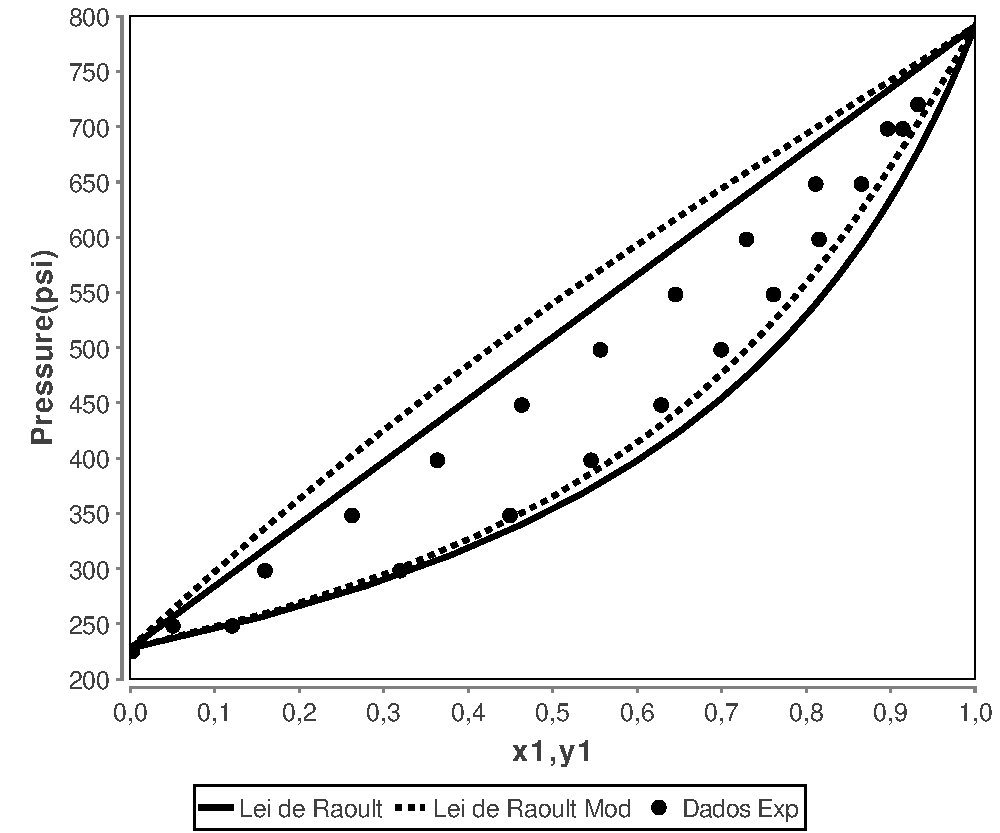
\includegraphics[width=0.8\textwidth]{img/VLE-Ethane(1)Propylene(2)-x1y1&Pressure-Raoult-RaoultMod.pdf}}
\caption{Diagrama de equilíbrio $P-xy$ da mistura de etano (1) e
propeno (2) calculados com as Leis de Raoul e Raoult Modificada utilizando
modelo de atividade UNIFAC(Do)}
\label{fig:raoult01}
\end{figure}

A \autoref{fig:raoult02} mostra um comparativo dos valores de fração molar da
fase gasosa e da fase líquida para o etano utilizando as leis de Raoult e Raoult
Modificado via UNIFAC (Do). Observa-se que as curvas ficaram distantes dos
pontos experimentais exceto para pressões mais baixas.

\begin{figure}[htb]
\centering
{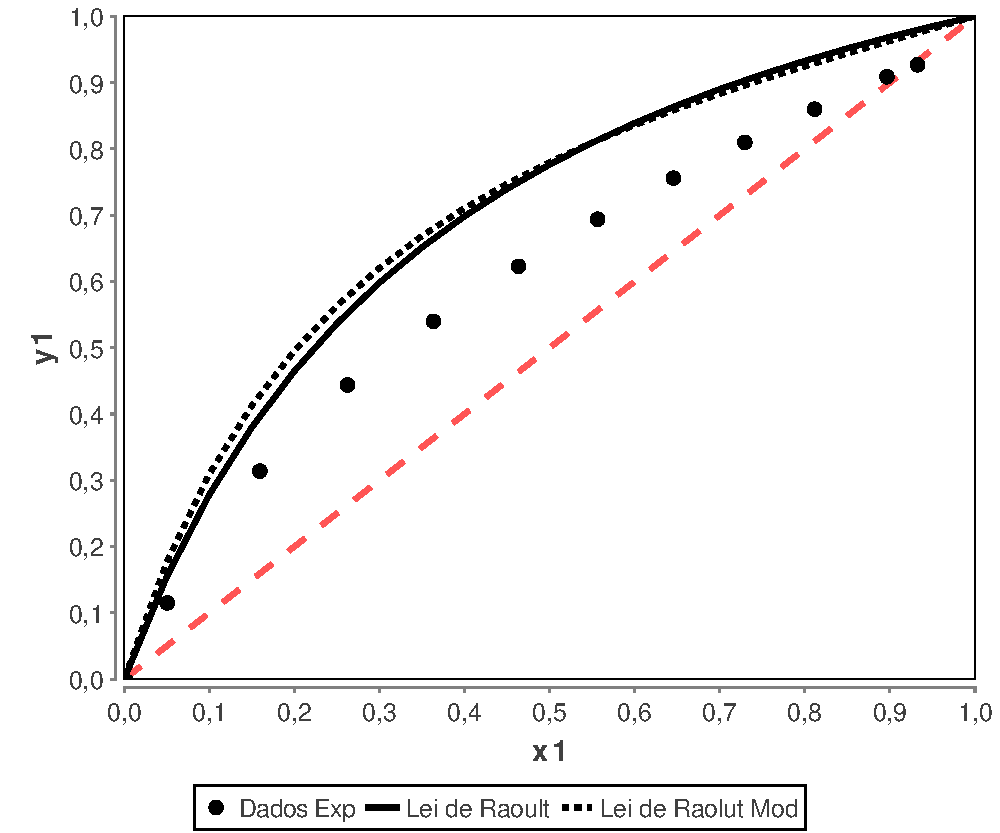
\includegraphics[width=0.8\textwidth]{img/VLE-Ethane(1)Propylene(2)-x1&y1-Raoult-RaoultMod.pdf}}
\caption{Diagrama de equilíbrio $y-x$ da mistura de etano (1) e
propeno (2) calculados com as Leis de Raoul e Raoult Modificada utilizando
modelo de atividade UNIFAC(Do)}
\label{fig:raoult02}
\end{figure} 


\subsection{Método $\phi-\phi$} 

As Figuras \ref{fig:phi01} e \ref{fig:phi02} apresentam a predição do método
$\phi-\phi$ utilizando Peng-Robinson como equação de estado para a mistura
etano e propeno. Apesar das mesmas não evidenciarem os valores
extremos, tais mostram que tal método obteve uma melhor predição dos valores
experimentais quando comparada àquelas mostradas nas Figuras
\ref{fig:raoult01} e \ref{fig:raoult02}.

\begin{figure}
\centering
{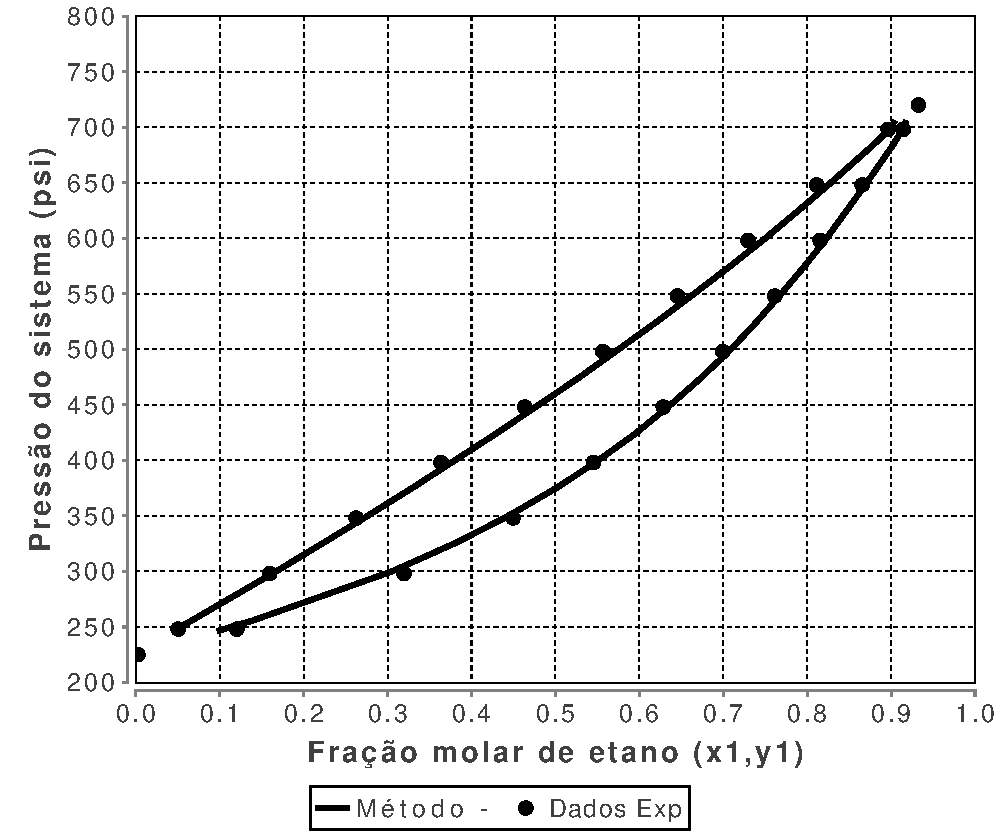
\includegraphics[width=0.8\textwidth]{img/VLE-Ethane(1)Propylene(2)-x1y1&Pressure-PengRobinson.pdf}}
\caption{Diagrama de equilíbrio $P-xy$ da mistura de de etano (1) e
prepeno (2) calculados com as EoSs PR}
\label{fig:phi01}
\end{figure}

\begin{figure}
\centering
{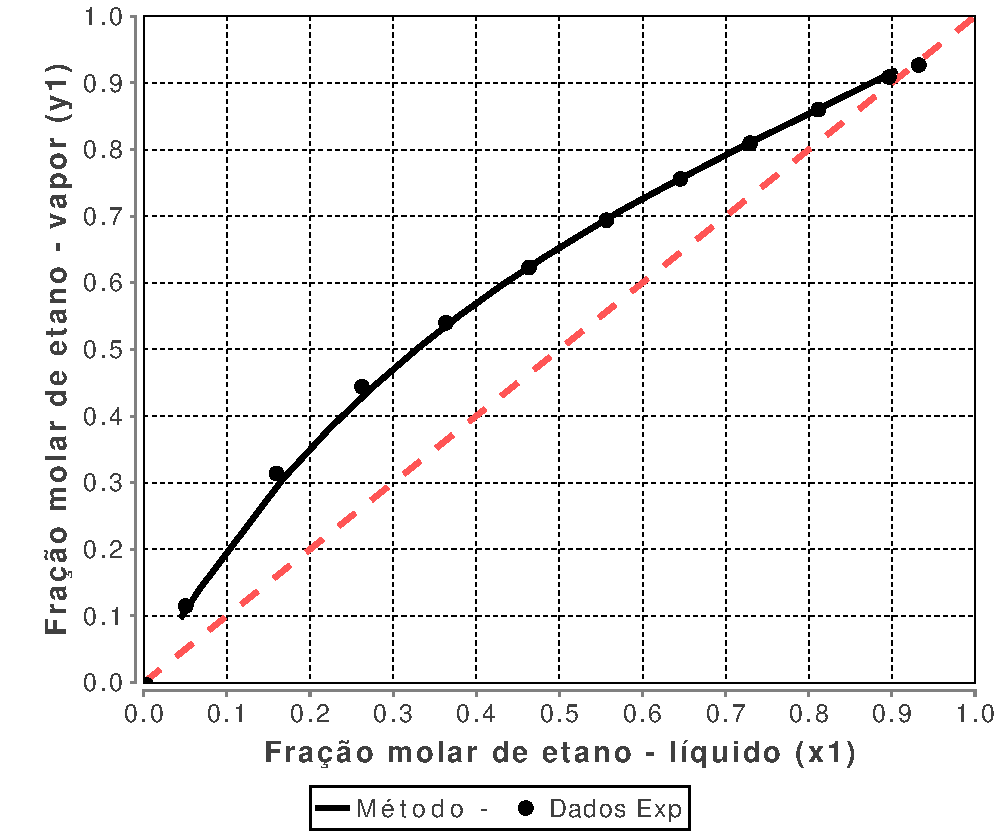
\includegraphics[width=0.8\textwidth]{img/VLE-Ethane(1)Propylene(2)-x1&y1-PengRobinson.pdf}}
\caption{Diagrama de equilíbrio $y-x$ da mistura de de etano (1) e
prepeno (2) calculados com as EoSs PR}
\label{fig:phi02}
\end{figure}
\clearpage

\section{Conclusões}

Este trabalho visou o estudo da predição e construção de diagramas de equílibrio
líquido-vapor (mistura etano e propeno) utilizando diferentes modelos de
cálculo. Foram utilizadas as Leis de Raoult e Raoult Modificada (com UNIFAC(Do)
para cálculo do coeficiente de atividade) e o modelo $\phi-\phi$ utilizando Peng-Robinson como equação de
estado e os valores preditos foram comparadas qualitativamente a dados
experimenais.

A partir dos resultados apresentados, conclui-se que o modelo $\phi-\phi$
preveu melhor os valores experimentais, visto que esse método considera ambas as
fases sendo não ideais. Tanto a lei de Raoult, como a lei de Raoult modificada,
apresentaram resultados menos satisfatórios para tais cálculos, sendo que a
primeira considera ambas as fases ideais e a segunda faz a consideração de
líquido não ideal. 

Os valores obtidos para o líquido, foram melhores aproximados pela lei de
Raoult Modificada. Já os do vapor, foram aproximados melhor através da Lei de Raoult.
Contudo, nenhum desses modelos foi capaz de prever o
comportamento supercrítico do etano.


  

 
 \newdimen\bibindent
\setlength\bibindent{1.5em} % identaçao das referencias
{ % Um lineskip menor neste contexto de referencias
\rhead{}
\baselineskip 4.3mm 
% Edite o arquivo bib.bib com as suas próprias referências 
\bibliography{bib}
} 
 
\end{document}
